This section provides a conceptual framework for understanding how birth spacing changes
and guiding the subsequent analysis.
I first introduce three potential explanations that link fertility and birth 
spacing decisions: economic conditions, desired child outcomes, and son preference 
\citep{Casterline2016,Portner2018}.
Next, I discuss why female education and area of residence are the principle factors 
in the empirical analyses and how they tie into the three explanations.

% Economic conditions
The improvements in economic condition, especially the doubling of real wages,
are likely to affect fertility although the direction is ambiguous, as, empirically, 
higher female wages lowers fertility, whereas higher male wages increases fertility 
\citep{Hotz1997,schultz97}.
Economic theory predicts that the effect of higher wages on fertility is determined by 
the relative strengths of the substitution and income effects.
The substitute effect captures that as wages increase time becomes more expensive, and
people therefore work more and spend less time on non-wage earning activities, such as 
children or leisure.
The income effect captures that higher wages increase the available income, which
leads people to spend more time on time-intensive activities and less time working.
Since women spend substantially more time on childrearing than men, the substitution effect 
dominates for women but the income effect for men.

If having children requires the mother to curtail her economic activities, higher
female wages, in addition to lowering fertility, will tend to shorten birth spacing.
Shortening birth spacing allows parents to take advantage of economies of scale in 
childrearing---for example, looking after two children simultaneously requires 
less than double the time needed to look after one child \citep{Vijverberg1982,Hotz1997}.


% Child outcomes
Parents care both about how many children they have and their outcomes, and with 
increasing returns to education and lower offspring mortality, parents are likely to 
reduce fertility and invest more in each child \citep{Rosenzweig1982a,Wolpin1997}.
The higher return to education means that parents have more of an incentive to 
invest in their children's education, which increases the cost of children and 
lowers fertility. 
Lower expected mortality means that fewer births are required to reach a 
desired number of surviving children and allow parents to invest more in each child.

Longer spacing between births is generally expected to have positive effects on 
child outcomes and if fertility falls because of increased desired for better child
outcomes we would also expect spacing to increase.
The clearest example of birth spacing affecting child outcomes is for health,
where very short spacing---approximately 24 months or less---leads to worse health 
and mortality outcomes for children 
\citep{Whitworth2002,Conde-Agudelo2012}.
Whether longer spacing also results in better human capital outcome is unclear as the 
evidence is mixed for developed countries and nonexistent for developing countries
\citep{Zajonc1976,Powell1993,Pettersson-Lidbom2009,Buckles2012,Barclay2017}.


% Son preference 
Empirically, a stronger son preference has only a minor effect on average fertility, but
son preference still affects the sex composition and fertility across families through 
differential stopping behavior and leads to shorter spacing and  worse health outcomes for 
daughters when there are no sons in the household 
\citep{repetto72,clark00,Whitworth2002,Basu2010,Jayachandran2011,Barcellos2014}.
 
Another result of son preference is the use of sex selection, which enables parents to 
avoid giving birth to a girl but increases the expected interval to the next birth
by 6--12 months for each abortion.
This increase consists of three parts. 
First, after an abortion, the uterus needs at least two menstrual cycles to recover, 
or the likelihood of spontaneous abortion increases substantially \citep{zhou00b}. 
Second, the waiting time to conception is one to six months. 
Finally, sex determination tests are reliable only from three months of gestation. 

The use of sex selection, and therefore the length of birth intervals, increases with
lower desired fertility and the higher the parity provided the desired number of sons has 
not been reached \citep{Portner2015b,Jayachandran2017}.  


% Factors/predictions
Although the explanations above are based on economic conditions, desired child outcome,
son preference, and the access to sex selection, none of these are available in the
data, so I instead use female education and area of residence as the two main explanatory 
variables in the empirical analyses.
Female education and area of residence are the closest available proxies and earlier 
research show that both higher female education and urbanization are associated with 
lower fertility and increased use of sex selection, and, therefore, likely also changes 
in birth spacing
\citep{das_gupta97,dreze01,bhat03,retherford03b,Guilmoto2009a,Portner2015b,Jayachandran2017}.
Furthermore, both variables are interesting given the tremendous increases in 
both education and urbanization in India; 
Figure \ref{fig:education_over_time} show the substantial increase in female education
in both rural and urban areas, although it is still considerably higher in urban than in 
rural areas and the proportion of the population living in urban areas almost doubled from 
18\% in 1960 to 35\% in 2019 \citep{United-Nations2019}.

\begin{figure}[htpb]
\centering
\subfloat[Rural]{
    \begin{minipage}{0.49\textwidth}
        
\includegraphics[width=\textwidth]{educ_over_time_rural}
    \end{minipage}
} 
\subfloat[Urban]{
    \begin{minipage}{0.49\textwidth}
        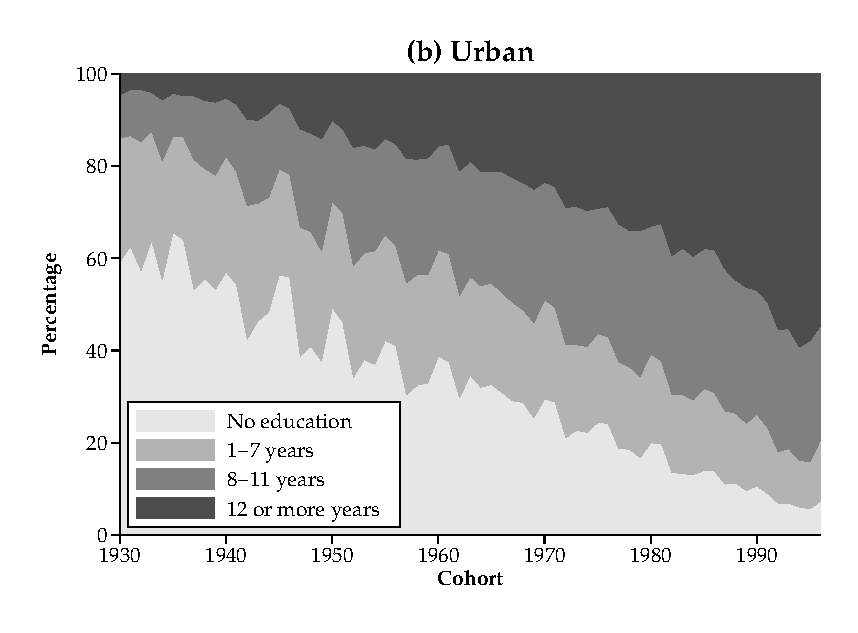
\includegraphics[width=\textwidth]{educ_over_time_urban} 
    \end{minipage}
}
\caption{Distribution of education by cohort for women 20 years or older
using the four rounds of the NFHS}
\label{fig:education_over_time}
\end{figure}


Women living in urban areas are likely to have lower fertility and higher use
of sex selection than women in rural areas.
The lower fertility is the result of higher cost of children and lower child mortality 
risk in urban compared to rural areas.%
\footnote{
However, holding parental education constant, there is evidence that children in
Indian slums do worse than they would have in rural areas \citep{Portner2018a}.
}
The higher use of sex selection comes partly from the lower fertility and partly from 
women in urban areas having higher income and better access to health care facilities.


As women receive more education their potential wages increase, which should shorten 
birth spacing and lower fertility, but the low and declining female labor force 
participation in India, especially for younger women, suggests that families face little 
incentive to space children more closely together for economic reasons.
Even as women's education increased, their labor force participation stagnated or 
decreased and is now one of the lowest outside the Middle East 
\citep{Klasen2015,Fletcher2017,Afridi2018,Bhargava2018,Chatterjee2018}.%
\footnote{
In line with other countries, there is still a U-shaped relationship between education and 
labor force participation for married women, with the lowest participation for 
women with 8--11 years of education \citep{Goldin1994,Chatterjee2018}.
See appendix Figures \ref{fig:work_by_survey} through \ref{fig:work_family_by_survey}. 
}

One explanation for the low female labor force participation is that male wages have 
increased so substantially that the income effect dominates any substitution effect.
The average male wage is almost 70\% higher than the female wage and women’s labor 
supply appears to be more negatively elastic to husbands' wages than positively elastic 
to their own wages \citep{Klasen2015,Bhargava2018}.

Furthermore, the increasing return to male education may make it appear as if higher 
female education results in lower fertility and more sex selection, if women with more 
education are better at producing child human capital as suggested by \citet{Behrman1999},.
The higher return to male education provides an additional incentive to invest in sons'
education, and one such investment is a better-educated mother.
As discussed above, the higher returns should also lower desired fertility, making the use 
of sex selection even more appealing, and possibly increases birth spacing.


% Sanskritization
Although the expansion in female education might bring in groups with initially different 
norms, the process of ``Sanskritization'' implies that as lower-castes females gain access 
to education, they adopt higher-caste norms such as stronger son preference and a retraction 
from the formal labor market \citep{Srinivas1956}.
The low and declining female labor force participation as husbands' wages increase 
indicates that this process still operates \citep{Abraham2013,Chatterjee2018}.

% Summary / hypotheses

In summary, with substantial increases in husbands' income and a declining female labor 
force participation, I expect longer birth spacing over time, independent of education 
levels.
Furthermore, birth spacing likely increases the most among the better educated 
because their household income increases the most---even with declining female labor 
participation---and because of their use of sex selection.
Finally, even with the substantial increase in the number of better-educated women, 
"Sanskritization" implies that the changing composition will not substantially change the 
use of sex selection.






